\graphicspath{ {./images/2_direct_current/} }

\chapter{Corriente y Resistencia}

\section{Corriente eléctrica}

Para comprender conceptualmente la corriente eléctrica o el flujo de cargas eléctricas es conveniente usar analogías. El movimiento de cargas en un conductor puede verse como un flujo de agua, es decir, partículas de agua atravesando una tubería. Manteniendo este carácter análogo, la cantidad de agua que fluye en un tubo se representa como caudal de agua. El caudal de agua se mide en unidad de volumen sobre unidad de tiempo, por ejemplo \unit{\cubic\metre\per\second}. Esto representa de una forma aproximada la cantidad de moléculas de \(\text{H}_2\text{O}\) que atraviesan una sección de tubo, ya que en un volumen dado, se puede determinar la cantidad de moléculas de agua para una cierta temperatura. Es evidente que \qty{1}{\cubic\metre} de agua contiene una cantidad enorme de moléculas, sin embargo, en términos simples, se cuantifica la \emph{cantidad de agua} que fluye por unidad de tiempo.

La idea para la corriente eléctrica es análoga a la corriente de agua. Se puede determinar la cantidad de cargas eléctricas libres que circulan por un conductor en un tiempo determinado. Así, se podría definir de forma intuitiva, que la corriente eléctrica o flujo de cargas eléctricas es la cantidad de cargas elementales que circulan por unidad de tiempo. Como la carga elemental tiene unidades de Coulomb, entonces las unidades de corriente deberían ser representadas en cantidad de Coulomb por segundo (\unit{\coulomb\per\second}). A continuación se realizará un análisis del movimiento de cargas en un conductor para verificar esta premisa.

\subsection{Movimiento de las cargas}
\label{sec:movimiento_de_cargas}

Para cualquier tipo de material conductor en condiciones normales y sin ningún tipo de fuerza eléctrica actuante, los electrones libres se mueven en direcciones aleatorias debido a la temperatura del material. Para que las cargas tengan un movimiento en una dirección determinada, es necesario que exista una fuerza que actúe sobre ellas. Esta fuerza es la fuerza eléctrica dada por la ley de Coulomb (ecuación \ref{eq:ley_coulomb}) que actúa sobre las cargas libres (electrones) debido a la presencia de un campo eléctrico \(\vec{E}\). Es decir, para que haya corriente eléctrica, debe existir un campo eléctrico que actúe sobre las cargas libres en el conductor. Este campo eléctrico puede ser generado por una diferencia de potencial entre dos puntos del conductor.

\begin{marginfigure}[-1cm]
  \centering
  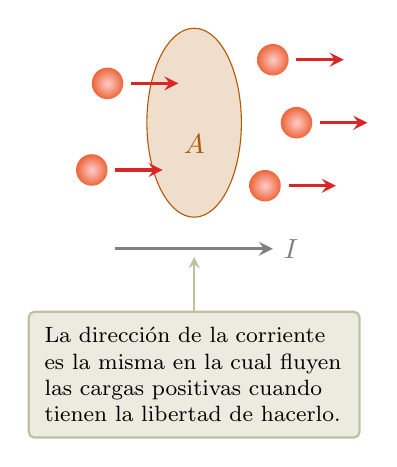
\begin{tikzpicture}[>=stealth]
  \draw[orange!70!black,fill=orange!70!black!20,name=conductor] (0,0) ellipse (0.6 and 1.2) node[below=0.8]{\(A\)};
  \draw[very thick,gray,->] (-1,-1.6) -- (1,-1.6) node[right]{\(I\)};

  \foreach \x\y in {-1.1/0.5,-1.3/-0.6,1/0.8,1.3/0,0.9/-0.8} {
    \shade[inner color=white!80!red, outer color=orange!50!red!70!lightgray] (\x,\y) circle (.2) [radius=1pt];
    \draw[very thick,color=red!70!gray,->] ({\x+0.3},\y) -- ({\x+0.9},\y);
  }

  \node (cartel) [
    font=\footnotesize,
    text width=3.8cm,
    align=left,
    fill=yellow!40!black!14,
    draw=yellow!40!black!46,
    thick,
    rounded corners=2pt,
    inner sep=2mm
    ]
    at (0,-3.2) {La dirección de la corriente es la misma en la cual fluyen las cargas positivas cuando tienen la libertad de hacerlo.};
  \draw[->, thick, color=yellow!40!black!46, shorten >=3pt] 
           (cartel.north) -- (0,-1.6);
\end{tikzpicture}

  \caption{Cargas en movimiento a través de un área \(A\).}
  \label{fig:current}
\end{marginfigure}
Cuando se aplica un campo eléctrico las cargas adquieren una velocidad como se muestra en la figura \ref{fig_cargas_libres}. Cuando se habla de velocidad, si se analiza una única partícula, se mide como cambia su posición con respecto al tiempo \(\vec{v}(t)=dx/dt\). Pero en un conductor no hay una sola partícula, sino miles de millones de electrones en movimiento. Para entender la corriente eléctrica observamos el desplazamiento de todo un ``bloque'' o volumen de carga. Las cargas en movimiento se analizan usando la velocidad de arrastre o velocidad de deriva \(v_d\) en la dirección del campo eléctrico. La velocidad de deriva es la velocidad promedio de las cargas. En un pequeño intervalo de tiempo \(dt\) las cargas avanzan una pequeña distancia \(dx\) en el conductor, y como \(v_d=dx/dt\) por definición de diferencial, se puede decir que la distancia que avanzan es 
\begin{equation}\label{eq_distancia_de_avance}
  dx=v_d\cdot dt
\end{equation}

\begin{tcolorbox}[myconclusion]
  La corriente se estudia a partir de la velocidad promedio \(v_d\) de las cargas debido a que una única carga aislada es difícil de estudiar. Al igual que sucede con las moléculas de agua al estudiar el caudal, se representa la velocidad de un volumen de agua mediante la velocidad promedio de las partículas que componen un volumen.
\end{tcolorbox}

Como se muestra en la figura \ref{fig_cargas_libres} las cargas en un conductor tienen una velocidad de deriva \(v_d\) y como se demostró en la expresión \eqref{eq_distancia_de_avance} la porción de distancia \(\Delta x\) que avanzan las cargas es \(v_d \cdot \Delta t\), que al ser pequeñas pueden considerarse diferenciales.

\marginnote{
  \begin{tcolorbox}[sidenote]\footnotesize{
      En este texto se ha usado \(\rho_c\) como la densidad volumétrica de cargas. No confunda esto con la resistividad \(\rho\). 

      En muchos casos se utiliza \(\rho_c=nq\) donde \(n\) es la cantidad de cargas libres y \(q\) es la carga eléctrica de cada carga libre. Ambas expresiones representan lo mismo.
    }
  \end{tcolorbox}
}
Al avanzar esa distancia \(dx\), todo ese ``bloque'' de electrones atraviesa el área transversal \(A\). El volumen de ese cilindro que acaba de cruzar la frontera es el área por la distancia 
\[
  dV=A \cdot dx
\]
Sustituyendo \(dx\) con la expresión \eqref{eq_distancia_de_avance}, resulta
\begin{equation}\label{eq_volumen_de_cargas}
  dV=A\cdot v_d \cdot dt
\end{equation}

\begin{figure}[!ht]
  \centering
  \input{chapters/2_direct_current/media/1_movimiento_de_cargas.tex}
  \caption{Movimiento de cargas en un conductor.}
  \label{fig_cargas_libres}
\end{figure}

Si se sabe que la cantidad de carga que hay por unidad de volumen, es decir, la densidad volumétrica de carga \(\rho_c\) del conductor, la cantidad total de carga \(dQ\) contenida en ese pequeño volumen \(dV\) que acaba de cruzar será:
\[
  dQ=\rho_c\cdot dV
\]
Si se sustituye \(dV\) con la expresión \eqref{eq_volumen_de_cargas} obtiene
\[
  dQ = \rho_c \cdot A \cdot v_d \cdot dt
\]

\marginnote{
  \begin{tcolorbox}[sidenote]\footnotesize{
      Es usual pensar que una variación de la carga en el tiempo significa que la carga del conductor cambia en el tiempo, pero cuidado, en este contexto \(Q\) no representa la carga del conductor, sino la carga que fluye por el.
    }
  \end{tcolorbox}
}
Si se toma esta última ecuación y se aplica la definición de diferencial, obtiene exactamente la definición de corriente 
\begin{equation}
  \boxed{
    I=\frac{dQ}{dt}=\rho_c\cdot A\cdot v_d
  }
\end{equation}
Así, puede ver que la corriente es directamente proporcional a la velocidad promedio a la que se desplazan las cargas, medido en Coulomb por segundo, tal y como se había anunciado al principio.

\begin{tcolorbox}[mydanger]
  La corriente eléctrica \(I\) es un valor escalar, a pesar de que se obtiene a partir de la velocidad de deriva, la carga \(dQ\) y el tiempo \(dt\) son escalares, y en consecuencia la corriente lo es. Más adelante se define la \emph{densidad de corriente} \(\vec{J}\) que representa la corriente con carácter vectorial.
\end{tcolorbox}

En el sistema internacional de unidades, se define la unidad de corriente como el amperio \unit{\ampere} que representa \qty{1}{\coulomb\per\second}.

\subsection{Corriente convencional}

La figura \ref{fig_corriente_convencional} presenta segmentos de material conductor. En la figura \ref{fig:flujo_de_cargas_positivas}, las cargas en movimiento son positivas, la fuerza eléctrica ocurre en la misma dirección que \(\vec{E}\), y la velocidad de deriva \(v_d\) es de izquierda a derecha. En la figura \ref{fig:flujo_de_cargas_negativas} las cargas son negativas, la fuerza eléctrica es opuesta a \(E\), y la velocidad de deriva \(v_d\) es de derecha a izquierda. Definimos que la corriente, denotada por \(I\), va en la dirección en la que hay un flujo de carga positiva. Por ello, las corrientes se describen como si consistieran por completo en un flujo de cargas positivas, aun en los casos en que se sabe que la corriente real se debe a electrones. Así, en las figuras \ref{fig:flujo_de_cargas_positivas} y \ref{fig:flujo_de_cargas_negativas} la corriente es hacia la derecha. Esta convención sobre la dirección del flujo de la corriente se llama \emph{corriente convencional}. Aunque la dirección de la corriente convencional no es necesariamente la misma en que se desplazan en realidad las partículas con carga, veremos que el signo de las cargas en movimiento tiene poca importancia en el análisis de los circuitos eléctricos.

\input{chapters/2_direct_current/media/1_corriente_convencional.tex}

A pesar de que en este apartado se habla de ``dirección de corriente'' siempre recuerde que la corriente es una magnitud \emph{escalar}. Por lo general describiremos la dirección de la corriente ya sea con palabras (por ejemplo, ``la corriente fluye por el circuito en el sentido horario'') o eligiendo una corriente como positiva si fluye en un sentido a lo largo de un conductor, y negativa si fluye en sentido contrario.

\subsection{Densidad de corriente}

Tal y como ocurre con el caudal de agua, la corriente eléctrica nada dice sobre la dirección o sentido del vector velocidad de las cargas. Si bien se puede otorgar una ``dirección'' verbalmente, matemáticamente hablando, la corriente es un escalar, y por tanto en una ecuación será un escalar. Esto puede limitar el estudio de la dinámica de las cargas en cierto punto. En un cable recto, la dirección es muy fácil de determinar, el signo del escalar será suficiente. Pero ¿qué sucedería si la corriente fluye a través de un material tridimensional con forma irregular, como una placa de metal o el océano? Para estudiar este tipo de fenómenos se requiere un campo vectorial. Para solucionar esto, en lugar de medir la corriente total a través de la superficie \(A\), se introduce una propiedad local y puntual que no depende de la geometría del cable. Así se busca describir lo que sucede con las cargas en un punto dado. 

De la sección anterior se sabe que la corriente para un área perpendicular al flujo de cargas es 
\[
  I=\rho_c \cdot A \cdot v_d
\]
Dividiendo ambos miembros por el área \(A\), se obtiene así la cantidad de corriente por unidad de área:
\[
  \frac{I}{A} = \rho_c \cdot v_d = J
\]
A esta magnitud se le denomina \emph{densidad de corriente}. Observe que en el miembro derecho, se tiene la velocidad de deriva \(v_d\) que tiene un carácter vectorial. En este caso \(J\) heredará ese carácter vectorial (\(I\) solo toma el módulo de \(v_d\)). Entonces, así ha definido formalmente el vector densidad de corriente 
\begin{equation}\label{eq_densidad_de_corriente}
  \vec{J}=\rho_c \vec{v}_d
\end{equation}
La densidad de corriente, en el sistema internacional, tiene unidades de \unit{\coulomb\per\second\per\metre\squared} o bien \unit{\ampere\per\metre\squared}. Es decir, el análisis dimensional sugiere que se está midiendo la cantidad de cargas que atraviesan una superficie de un metro cuadrado en un segundo. 

\begin{tcolorbox}[myconclusion]
  Observe que aquí toma sentido el hecho de que \(dQ\) no es la carga del cable, sino la carga que fluye a través de el. Esto, se puede deducir de la siguiente manera: La densidad de corriente \(\vec{J}\) no establece ninguna relación con la carga del conductor, sino 
  \[
    \vec{J}=\rho_c \vec{v}_d = \rho_c\frac{d\vec{r}}{dt}
  \]
  una relación con la tasa de cambio de la posición \(\vec{r}\) de una densidad de carga \(\rho_c\) en el tiempo. Es decir, es la velocidad multiplicada por la densidad volumétrica de carga del material.
\end{tcolorbox}

En este momento, si ha sido perspicaz al leer la deducción de la densidad de corriente, tal vez le resulte un poco extraño el hecho de que a pesar de que \(\vec{J}\) es una cantidad vectorial, no parece dar mucha información del comportamiento interno en el conductor, es decir, del movimiento de cargas. Es más, al introducir este tópico, se menciona justamente que esta es la herramienta que nos permite analizar el comportamiento de la corriente eléctrica con carácter vectorial en situaciones donde la cantidad \(I\) no es suficiente.

En la deducción de la densidad de corriente, cuando divide por el área total \(A\), lo que realmente se busca es pasar de una propiedad macroscópica a una microscópica. Al dividir \(I\) entre \(A\), asumiendo que la corriente se distribuye uniformemente por todo el cable, se está encontrando una propiedad de cada partícula individual, ya que el área puede tomarse tan pequeña como se quiera. Es decir, puede utilizar diferenciales de área \(dA\) para analizar pequeñas partes del flujo de cargas. Esto resulta en 
\[
  dI = \vec{J}\cdot d\vec{A}
\]
Y de este diferencial se puede obtener el comportamiento individual de cada carga en movimiento. Como \(J\) y \(A\) son vectores y \(I\) es un escalar se usa el producto escalar. Esto implica que para cada diferencial de área, se tiene en cuenta el ángulo con el que las cargas atraviesan cualquier superficie. Realizando una integral sobre una superficie \(S\) de la densidad de corriente \(\vec{J}\) con respecto a un diferencial de área,
\[
  I = \iint_S \vec{J}\cdot d\vec{A}
\]
se logra obtener la corriente incluso para casos donde la corriente no se distribuye de forma uniforme. El gran beneficio de esto es que \(\vec{J}\) permite recuperar la corriente porque conoce el comportamiento de cada carga.

\section{Ley de Ohm}

El físico alemán George Simon Ohm descubrió empíricamente la relación que existe entre la corriente eléctrica, la diferencia de potencial y la resistencia del material. 

En la época de George Ohm aún no se conocía la existencia del electrón. Ohm experimentaba con termopares, donde al mantener una diferencia de temperatura en los extremos de dos metales distintos, se generaba una diferencia de potencial. Conectó cables de diferentes longitudes y grosores a su circuito y midió la fuerza magnética generada por la corriente. Al graficar sus datos, se dio cuenta de que la corriente era inversamente proporcional a la longitud del cable y directamente proporcional a la sección transversal. Descubrió experimentalmente la resistencia y formuló la relación macroscópica que hoy conocemos.

En nuestro estudio, podemos realizar experimentos para comprobar la validez de esta ley, sin embargo, la ventaja de el análisis matemático es que se puede modelar este fenómeno y llegar a la ley de Ohm de una forma puramente analítica. En este contexto se utilizará el llamado modelo de Drude para encontrar la ley de Ohm.

\subsection{Modelo de Drude}

El modelo de Drude, propuesto en 1900, asume que los electrones rebotan contra los átomos del material, como si fueran bolas en una máquina de pinball. 

Cuando se aplica un campo eléctrico \(E\), una carga libre \(q\) experimenta una fuerza eléctrica,
\[
  F=qE
\]
Por la segunda ley de Newton, esta fuerza produce una aceleración:
\[
  a=\frac{qE}{m}
\]
donde \(m\) es la masa del portador de carga.

Si los electrones solo aceleran, su velocidad tendería a infinito. Pero en la realidad, chocan constantemente con la red cristalina del material. Se define \(\tau\) (tau) como el \emph{tiempo de relajación} que es el tiempo promedio entre colisiones.

Después de cada colisión, el electrón pierde su velocidad dirigida, y vuelve a ser acelerado por el campo. Por lo tanto, la velocidad promedio \(v_d\) que alcanzan es la aceleración multiplicada por este tiempo de relajación:
\begin{equation}\label{eq_vd_tiempo_de_relajacion}
  v_d = a\tau = \frac{qE\tau}{m}
\end{equation}

Ahora, partiendo de la densidad de carga \(J\), 
\[
  J=\rho_c v_d
\]
se puede sustituir \(v_d\) con la expresión de la ecuación \eqref{eq_vd_tiempo_de_relajacion} resultando 
\[
  J=\rho_c \frac{qE\tau}{m}
\]
Como \(\rho_c=nq\), donde \(n\) es la cantidad de cargas libres del material y \(q\) la carga de cada portador libre, entonces esta última expresión se puede escribir agrupando términos,
\[
  J=\left(\frac{nq^2 \tau}{m}\right) E
\]

Toda la expresión entre paréntesis está compuesta por propiedades intrínsecas del material (la densidad de carga, la carga del electrón, el tiempo entre colisiones y la masa del electrón). A todo este bloque se le denomina \emph{conductividad eléctrica} \(\sigma\):
\[
  \sigma = \frac{nq^2\tau}{m}
\]
Entonces la expresión de la densidad de corriente eléctrica puede reescribirse usando la conductividad, resultando en la Ley de Ohm:
\begin{equation}\label{eq_ley_de_ohm}
  J=\sigma E
\end{equation}

\subsection{Ley de Ohm macroscópica}

En base a la ecuación \eqref{eq_ley_de_ohm} se puede obtener una relación de parámetros macroscópicos en un circuito. Para ello se van a establecer las condiciones de un circuito ideal para poder modelarlo. Imagine un hilo conductor cilíndrico que tiene una longitud \(\ell\) y un área de sección transversal \(A\). La densidad de corriente \(J\) es la cantidad de corriente que atraviesa una unidad de área. Si se asume que la corriente se distribuye uniformemente por toda la sección transversal del cable, la corriente total \(I\) es simplemente el producto de la densidad de corriente por el área:
\[
  I=JA \quad \text{entonces} \quad J=\frac{I}{A}
\]

Por otro lado, si se asume un campo eléctrico uniforme en el hilo conductor, la diferencia de potencial \(\Delta V\) entre los extremos del cable está relacionada con el campo eléctrico y la distancia 
\[
  \Delta V = E\ell \quad \text{entonces} \quad E = \frac{\Delta V}{\ell}
\]

Con estas dos relaciones, se puede tomar la expresión \eqref{eq_ley_de_ohm} y sustituir la densidad de corriente y el campo eléctrico por las respectivas cantidades,
\[
  J=\sigma E \quad \rightarrow \quad \frac{I}{A}=\sigma \frac{\Delta V}{\ell}
\]
Operando algebráicamente,
\[
  \Delta V = I \left(\frac{\ell}{\sigma A}\right)
\]
Donde se define la expresión entre paréntesis como resistencia del material, y se denota con la letra \(R\). Así, la ley de Ohm macroscópica resulta ser 
\[
  \Delta V = IR
\]
\begin{tcolorbox}[myconclusion]
  En la practica se suele denotar a la diferencia de potencial \(\Delta V\) simplemente como \(V\).

  Además, en vez de utilizarse la conductividad \(\sigma\), suele emplearse la resistividad \(\rho\) del material, que es el inverso de la conductividad:
  \[
    \rho = \frac{1}{\sigma}
  \]
  ya que experimentalmente es más conveniente determinar la resistividad que la conductividad.
\end{tcolorbox}

\section{Aplicación de la ley de Ohm a circuitos}

\subsection{Circuitos en Serie}

Antes de comenzar es importante tener en cuenta que en un circuito en serie la corriente \( I \) es la misma en todos los elementos debido a que no hay bifurcaciones. Esto es debido a la conservación de la carga eléctrica y a la naturaleza de la conexión en serie.

Para entenderlo desde un enfoque físico, cuando varios elementos (resistencias, capacitores, etc.) están conectados en serie, sólo hay un camino posible para que circule la corriente eléctrica. Esto significa que las cargas eléctricas (generalmente electrones en un conductor metálico) no tienen bifurcaciones o alternativas en su trayecto: todas las cargas que pasan por un punto del circuito deben pasar por todos los demás puntos sucesivos en la misma rama.

Aplicando la ley de conservación de la carga (una consecuencia directa de la ley de continuidad en electromagnetismo), se deduce que no puede haber acumulación de carga en ningún punto del conductor en estado estacionario. Por tanto, el flujo de carga (es decir, la corriente) debe ser constante en todos los elementos conectados en serie. Si no fuera así, habría acumulación o desaparición de carga en algún nodo, lo cual no ocurre en un circuito cerrado en régimen permanente.

Es como el flujo de agua en una fuente; el agua brota de la parte superior de la fuente al mismo ritmo con el que llega a la parte inferior, sin importar las dimesiones de la fuetne. ¡El agua no ``se gasta'' a lo largo del trayecto!

En base a esta premisa, para cada resistencia, se cumple:
\[
  V_i = I R_i
\]

La ley de Kirchhoff de tensiones establece que la suma de las caídas de potencial en una malla cerrada es igual a la fuente de tensión aplicada:
\[
  V = V_1 + V_2 + \cdots + V_n = IR_1 + IR_2 + \cdots + IR_n
\]

Factorizando la corriente \( I \):
\[
  V = I (R_1 + R_2 + \cdots + R_n)
\]

Definiendo la resistencia equivalente \( R_{\text{eq}} \) del sistema:
\[
  \boxed{R_{\text{eq}} = R_1 + R_2 + \cdots + R_n}
\]

\paragraph{Ejemplo sencillo:}

Tres resistencias: \( R_1 = 2 \, \Omega \), \( R_2 = 3 \, \Omega \), \( R_3 = 5 \, \Omega \)
\[
  R_{\text{eq}} = 2 + 3 + 5 = 10 \, \Omega
\]
Si se aplica una diferencia de potencial de \( V = 20 \, \text{V} \), entonces:
\[
  I = \frac{V}{R_{\text{eq}}} = \frac{20}{10} = 2 \, \text{A}
\]

\subsection{Circuitos en Paralelo}

Al igual que en la sección anterior, vamos a partir con algunos supuestos físicos:
\begin{itemize}
  \item Las resistencias \( R_1, R_2, \dots,R_n \) están conectadas en paralelo tienen sus terminales conectadas a los mismos dos nodos.
  \item La diferencia de potencial \( V \) es la misma en cada una.
  \item La corriente total se divide entre las ramas: \( I = I_1 + I_2 + \cdots + I_n \)
\end{itemize}

Entonces, aplicando la ley de Ohm y de la ley de Kirchhoff de corrientes

En cada resistencia, se cumple:
\[
  I_i = \frac{V}{R_i}
\]
La corriente total será:
\[
  I = \frac{V}{R_1} + \frac{V}{R_2} + \cdots + \frac{V}{R_n}
\]
Factorizando \( V \):
\[
  I = V \left( \frac{1}{R_1} + \frac{1}{R_2} + \cdots + \frac{1}{R_n} \right)
\]
Definimos \( R_{\text{eq}} \) como la resistencia que satisface \( I = \frac{V}{R_{\text{eq}}} \). Entonces:
\[
  \frac{V}{R_{\text{eq}}} = V \left( \sum_{i=1}^{n} \frac{1}{R_i} \right)
  \Rightarrow \boxed{\frac{1}{R_{\text{eq}}} = \frac{1}{R_1} + \frac{1}{R_2} + \cdots + \frac{1}{R_n}}
\]

\paragraph{Ejemplo sencillo:}

Tres resistencias: \( R_1 = 4 \, \Omega \), \( R_2 = 6 \, \Omega \), \( R_3 = 12 \, \Omega \)

\[
  \frac{1}{R_{\text{eq}}} = \frac{1}{4} + \frac{1}{6} + \frac{1}{12} = \frac{3 + 2 + 1}{12} = \frac{6}{12} = \frac{1}{2}
  \Rightarrow R_{\text{eq}} = 2 \, \Omega
\]

\section{Energía y Potencia eléctrica}

Ahora abordaremos las expresiones teóricas de energía y potencia eléctrica en un circuito de corriente continua, partiendo de principios fundamentales. Estas magnitudes están directamente relacionadas con el trabajo que realiza el campo eléctrico sobre las cargas en movimiento. 

\subsection{Trabajo eléctrico}

Recordando lo que vimos en la unidad de electrostática, cuando una carga eléctrica \( q \) se desplaza entre dos puntos con diferencia de potencial \( \Delta V \), el trabajo realizado por el campo eléctrico es:
\[
  W = q \Delta V
\]

Este trabajo es la energía transferida al sistema. Si en lugar de una sola carga \(q\) consideramos una corriente continua \( I \), que representa el flujo de carga por unidad de tiempo podríamos calcular el trabajo realizado por la corriente de cargas, entonces partir de la definición de corriente operamos para obtener una expresión para \(q\):

\begin{align*}
  I &= \frac{\Delta q}{\Delta t} \\
  I \Delta t &= \Delta q \\
  \Delta q &= I \Delta t
\end{align*}

Entonces, el trabajo realizado en ese intervalo de tiempo es:

\begin{equation}
  W = I \Delta V \, \Delta t
  \label{eq:trabajo_electrico}    
\end{equation}

\subsection{Potencia eléctrica}

La potencia es el trabajo realizado en un intervalo de tiempo, entonces la tasa de transferencia de energía (o trabajo realizado) por unidad de tiempo es:
\[
  P = \frac{dW}{dt}
\]
Sustituyendo la expresión anterior para \( W \), obtenemos:
\begin{align}
  P &= \frac{d}{dt}(I \Delta V \, \Delta t) = I \Delta V \notag \\
  P &= IV
\end{align}
Esta expresión nos indica la potencia disipada (si \( V \) e \( I \) tienen el mismo signo) o suministrada (si tienen signos opuestos) en un componente del circuito.

Aplicando la ley de Ohm (\( V = IR \)) a la ecuación de potencia podemos encontrar la potencia disipada en una resistencia:
\[
  P = VI = (IR)I = \boxed{P = I^2 R}
\]
Alternativamente, despejando la corriente de la ley de Ohm:
\[
  I = \frac{V}{R} \Rightarrow P = V \left( \frac{V}{R} \right) = \boxed{P = \frac{V^2}{R}}
\]
Estas tres expresiones son equivalentes:
\begin{equation}
  \boxed{P = VI = I^2 R = \frac{V^2}{R}}
  \label{eq:potencia_electrica}
\end{equation}
y se usan dependiendo de qué variables sean conocidas en un circuito dado.

\subsection{Energía disipada en el tiempo}

Integrando la potencia en el tiempo se obtiene la energía total disipada o entregada:
\[
  W = \int_{t_0}^{t_1} P \, dt = \int_{t_0}^{t_1} VI \, dt
\]
Si el circuito opera bajo condiciones constantes (circuito de corriente continua pura), entonces:
\[
  W = V I \Delta t
\]
Si la resistencia es la única componente significativa, entonces:
\[
  W = I^2 R \Delta t = \frac{V^2}{R} \Delta t
\]

\paragraph{Ejemplo sencillo}

Un resistor de \( R = 10 \, \Omega \) conectado a una batería de \( V = 12 \, \text{V} \), durante \( \Delta t = 30 \, \text{s} \).
\begin{itemize}
  \item Corriente: \( I = \frac{V}{R} = \frac{12}{10} = 1.2 \, \text{A} \)
  \item Potencia disipada: \( P = I^2 R = (1.2)^2 \cdot 10 = 14.4 \, \text{W} \)
  \item Energía disipada: \( W = P \Delta t = 14.4 \cdot 30 = 432 \, \text{J} \)
\end{itemize}

\section{Resumen}
Resumen final de ecuaciones clave

\begin{tcolorbox}[title=Corriente Eléctrica]
  La corriente eléctrica es la tasa a la cual circula la carga a traves de una superficie.
  \[
    I_{prom} = \frac{\Delta Q}{\Delta t}
  \]
  que puede relacionarse con el movimiento de las cargas:
  \[
    I_{prom} = n q v_d A
  \]

  De esta ecuación se puede obtener la velocidad a la cual circulan los portadores de carga. La velocidad de deriva o arrastre es:
  \[
    v_d = \frac{I}{nqA}
  \]
  donde:
  \begin{itemize}
    \item \(I\) es la corriente que circula por el material
    \item \(q\) es la carga de los portadores (\(e=1.6\times10^{-19}\) en el caso de los electrones)
    \item \(A\) es el área transversal del material
    \item \(n\) es la densidad de portadores (el número de portadores) del el material por unidad de volumen.
  \end{itemize}

  Para obtener \(n\) para un material dado podemos usar la siguiente aproximación:
  \[
    n=\frac{\delta}{m_{molar}} N_A
  \]
  donde:
  \begin{itemize}
    \item \(\delta\) es la densidad del material
    \item \(m_{molar}\) es la masa molar del material
    \item \(N_A = 6.022 \times 10^{23} \, \mathrm{mol}^{-1}\) es el número de Avogadro.
  \end{itemize}
\end{tcolorbox}

\begin{tcolorbox}[title=Ley de Ohm]
  La ley de Ohm establece una relación de proporcionalidad entre la corriente, el potencial y la resistencia:
  \[
    V = IR
  \]
  \begin{itemize}
    \item La densidad de corriente es: \(\vec{J} = \sigma \vec{E}\)
    \item Ley de Ohm macroscópica: \(I = \frac{\sigma A}{L} \Delta V\)
    \item Definición de resistencia: \(R = \frac{\Delta V}{I} = \rho \frac{L}{A}\)
    \item Relación entre corriente y densidad de corriente: \(I = \int_A \vec{J} \cdot d\vec{A}\)
  \end{itemize}
  Estas ecuaciones permiten modelar y analizar cualquier sistema de corriente continua en conductores ohmicos.
\end{tcolorbox}


\begin{tcolorbox}[title=Circuitos]
  \paragraph{Serie:}
  \begin{itemize}
    \item Corriente común: \( I = \text{constante} \)
    \item Tensión total: \( V = V_1 + V_2 + \cdots + V_n \)
    \item Resistencia equivalente: \(R_{\text{eq}} = \sum_{i=1}^{n} R_i\)
  \end{itemize}
  
  \paragraph{Paralelo:}
  \begin{itemize}
    \item Tensión común: \( V = \text{constante} \)
    \item Corriente total: \( I = I_1 + I_2 + \cdots + I_n \)
    \item Resistencia equivalente: \(\frac{1}{R_{\text{eq}}} = \sum_{i=1}^{n} \frac{1}{R_i}\)
  \end{itemize}
\end{tcolorbox}


\begin{tcolorbox}[title=Trabajo y Potencia eléctrica]
  \paragraph{Potencia general:}  
  
  \[
    P = V I
  \]
  
  \paragraph{Potencia disipada en resistencias:}  
  \[
    P = I^2 R = \frac{V^2}{R}
  \]
  
  \paragraph{Energía disipada o entregada en el tiempo \( \Delta t \):}
  \[
    W = P \Delta t = V I \Delta t = I^2 R \Delta t = \frac{V^2}{R} \Delta t
  \]
\end{tcolorbox}

